%% bare_conf.tex
%% V1.3
%% 2007/01/11
%% by Michael Shell
%% See:
%% http://www.michaelshell.org/
%% for current contact information.
%%
%% This is a skeleton file demonstrating the use of IEEEtran.cls
%% (requires IEEEtran.cls version 1.7 or later) with an IEEE conference paper.
%%
%% Support sites:
%% http://www.michaelshell.org/tex/ieeetran/
%% http://www.ctan.org/tex-archive/macros/latex/contrib/IEEEtran/
%% and
%% http://www.ieee.org/

%%*************************************************************************
%% Legal Notice:
%% This code is offered as-is without any warranty either expressed or
%% implied; without even the implied warranty of MERCHANTABILITY or
%% FITNESS FOR A PARTICULAR PURPOSE! 
%% User assumes all risk.
%% In no event shall IEEE or any contributor to this code be liable for
%% any damages or losses, including, but not limited to, incidental,
%% consequential, or any other damages, resulting from the use or misuse
%% of any information contained here.
%%
%% All comments are the opinions of their respective authors and are not
%% necessarily endorsed by the IEEE.
%%
%% This work is distributed under the LaTeX Project Public License (LPPL)
%% ( http://www.latex-project.org/ ) version 1.3, and may be freely used,
%% distributed and modified. A copy of the LPPL, version 1.3, is included
%% in the base LaTeX documentation of all distributions of LaTeX released
%% 2003/12/01 or later.
%% Retain all contribution notices and credits.
%% ** Modified files should be clearly indicated as such, including  **
%% ** renaming them and changing author support contact information. **
%%
%% File list of work: IEEEtran.cls, IEEEtran_HOWTO.pdf, bare_adv.tex,
%%                    bare_conf.tex, bare_jrnl.tex, bare_jrnl_compsoc.tex
%%*************************************************************************

% *** Authors should verify (and, if needed, correct) their LaTeX system  ***
% *** with the testflow diagnostic prior to trusting their LaTeX platform ***
% *** with production work. IEEE's font choices can trigger bugs that do  ***
% *** not appear when using other class files.                            ***
% The testflow support page is at:
% http://www.michaelshell.org/tex/testflow/



% Note that the a4paper option is mainly intended so that authors in
% countries using A4 can easily print to A4 and see how their papers will
% look in print - the typesetting of the document will not typically be
% affected with changes in paper size (but the bottom and side margins will).
% Use the testflow package mentioned above to verify correct handling of
% both paper sizes by the user's LaTeX system.
%
% Also note that the "draftcls" or "draftclsnofoot", not "draft", option
% should be used if it is desired that the figures are to be displayed in
% draft mode.
%
\documentclass[conference]{IEEEtran}
% Add the compsoc option for Computer Society conferences.
%
% If IEEEtran.cls has not been installed into the LaTeX system files,
% manually specify the path to it like:
% \documentclass[conference]{../sty/IEEEtran}

% Some very useful LaTeX packages include:
% (uncomment the ones you want to load)

% *** MISC UTILITY PACKAGES ***
%
%\usepackage{ifpdf}
% Heiko Oberdiek's ifpdf.sty is very useful if you need conditional
% compilation based on whether the output is pdf or dvi.
% usage:
% \ifpdf
%   % pdf code
% \else
%   % dvi code
% \fi
% The latest version of ifpdf.sty can be obtained from:
% http://www.ctan.org/tex-archive/macros/latex/contrib/oberdiek/
% Also, note that IEEEtran.cls V1.7 and later provides a builtin
% \ifCLASSINFOpdf conditional that works the same way.
% When switching from latex to pdflatex and vice-versa, the compiler may
% have to be run twice to clear warning/error messages.

% *** CITATION PACKAGES ***
%
%\usepackage{cite}
\usepackage{cite}
% cite.sty was written by Donald Arseneau
% V1.6 and later of IEEEtran pre-defines the format of the cite.sty package
% \cite{} output to follow that of IEEE. Loading the cite package will
% result in citation numbers being automatically sorted and properly
% "compressed/ranged". e.g., [1], [9], [2], [7], [5], [6] without using
% cite.sty will become [1], [2], [5]--[7], [9] using cite.sty. cite.sty's
% \cite will automatically add leading space, if needed. Use cite.sty's
% noadjust option (cite.sty V3.8 and later) if you want to turn this off.
% cite.sty is already installed on most LaTeX systems. Be sure and use
% version 4.0 (2003-05-27) and later if using hyperref.sty. cite.sty does
% not currently provide for hyperlinked citations.
% The latest version can be obtained at:
% http://www.ctan.org/tex-archive/macros/latex/contrib/cite/
% The documentation is contained in the cite.sty file itself.


% *** GRAPHICS RELATED PACKAGES ***
%
\ifCLASSINFOpdf
  % \usepackage[pdftex]{graphicx}
  % declare the path(s) where your graphic files are
  % \graphicspath{{../pdf/}{../jpeg/}}
  % and their extensions so you won't have to specify these with
  % every instance of \includegraphics
  % \DeclareGraphicsExtensions{.pdf,.jpeg,.png}
\else
  % or other class option (dvipsone, dvipdf, if not using dvips). graphicx
  % will default to the driver specified in the system graphics.cfg if no
  % driver is specified.
   \usepackage[dvips]{graphicx}
  % declare the path(s) where your graphic files are
   \graphicspath{{../figures/}}
  % and their extensions so you won't have to specify these with
  % every instance of \includegraphics
   \DeclareGraphicsExtensions{.eps}
\fi
% graphicx was written by David Carlisle and Sebastian Rahtz. It is
% required if you want graphics, photos, etc. graphicx.sty is already
% installed on most LaTeX systems. The latest version and documentation can
% be obtained at: 
% http://www.ctan.org/tex-archive/macros/latex/required/graphics/
% Another good source of documentation is "Using Imported Graphics in
% LaTeX2e" by Keith Reckdahl which can be found as epslatex.ps or
% epslatex.pdf at: http://www.ctan.org/tex-archive/info/
%
% latex, and pdflatex in dvi mode, support graphics in encapsulated
% postscript (.eps) format. pdflatex in pdf mode supports graphics
% in .pdf, .jpeg, .png and .mps (metapost) formats. Users should ensure
% that all non-photo figures use a vector format (.eps, .pdf, .mps) and
% not a bitmapped formats (.jpeg, .png). IEEE frowns on bitmapped formats
% which can result in "jaggedy"/blurry rendering of lines and letters as
% well as large increases in file sizes.
%
% You can find documentation about the pdfTeX application at:
% http://www.tug.org/applications/pdftex


% *** MATH PACKAGES ***
%
\usepackage[cmex10]{amsmath}
% A popular package from the American Mathematical Society that provides
% many useful and powerful commands for dealing with mathematics. If using
% it, be sure to load this package with the cmex10 option to ensure that
% only type 1 fonts will utilized at all point sizes. Without this option,
% it is possible that some math symbols, particularly those within
% footnotes, will be rendered in bitmap form which will result in a
% document that can not be IEEE Xplore compliant!
%
% Also, note that the amsmath package sets \interdisplaylinepenalty to 10000
% thus preventing page breaks from occurring within multiline equations. Use:
%\interdisplaylinepenalty=2500
% after loading amsmath to restore such page breaks as IEEEtran.cls normally
% does. amsmath.sty is already installed on most LaTeX systems. The latest
% version and documentation can be obtained at:
% http://www.ctan.org/tex-archive/macros/latex/required/amslatex/math/





% *** SPECIALIZED LIST PACKAGES ***
%
%\usepackage{algorithmic}
% algorithmic.sty was written by Peter Williams and Rogerio Brito.
% This package provides an algorithmic environment fo describing algorithms.
% You can use the algorithmic environment in-text or within a figure
% environment to provide for a floating algorithm. Do NOT use the algorithm
% floating environment provided by algorithm.sty (by the same authors) or
% algorithm2e.sty (by Christophe Fiorio) as IEEE does not use dedicated
% algorithm float types and packages that provide these will not provide
% correct IEEE style captions. The latest version and documentation of
% algorithmic.sty can be obtained at:
% http://www.ctan.org/tex-archive/macros/latex/contrib/algorithms/
% There is also a support site at:
% http://algorithms.berlios.de/index.html
% Also of interest may be the (relatively newer and more customizable)
% algorithmicx.sty package by Szasz Janos:
% http://www.ctan.org/tex-archive/macros/latex/contrib/algorithmicx/




% *** ALIGNMENT PACKAGES ***
%
\usepackage{array}
\usepackage{tabularx,ragged2e,booktabs}
% Frank Mittelbach's and David Carlisle's array.sty patches and improves
% the standard LaTeX2e array and tabular environments to provide better
% appearance and additional user controls. As the default LaTeX2e table
% generation code is lacking to the point of almost being broken with
% respect to the quality of the end results, all users are strongly
% advised to use an enhanced (at the very least that provided by array.sty)
% set of table tools. array.sty is already installed on most systems. The
% latest version and documentation can be obtained at:
% http://www.ctan.org/tex-archive/macros/latex/required/tools/


%\usepackage{mdwmath}
%\usepackage{mdwtab}
% Also highly recommended is Mark Wooding's extremely powerful MDW tools,
% especially mdwmath.sty and mdwtab.sty which are used to format equations
% and tables, respectively. The MDWtools set is already installed on most
% LaTeX systems. The lastest version and documentation is available at:
% http://www.ctan.org/tex-archive/macros/latex/contrib/mdwtools/


% IEEEtran contains the IEEEeqnarray family of commands that can be used to
% generate multiline equations as well as matrices, tables, etc., of high
% quality.


%\usepackage{eqparbox}
% Also of notable interest is Scott Pakin's eqparbox package for creating
% (automatically sized) equal width boxes - aka "natural width parboxes".
% Available at:
% http://www.ctan.org/tex-archive/macros/latex/contrib/eqparbox/

% *** SUBFIGURE PACKAGES ***
%\usepackage[font={small}]{caption, subfig}
\usepackage[font=footnotesize]{caption, subfig}
%\usepackage[tight,footnotesize]{subfigure}
% subfigure.sty was written by Steven Douglas Cochran. This package makes it
% easy to put subfigures in your figures. e.g., "Figure 1a and 1b". For IEEE
% work, it is a good idea to load it with the tight package option to reduce
% the amount of white space around the subfigures. subfigure.sty is already
% installed on most LaTeX systems. The latest version and documentation can
% be obtained at:
% http://www.ctan.org/tex-archive/obsolete/macros/latex/contrib/subfigure/
% subfigure.sty has been superceeded by subfig.sty.



%\usepackage{caption}
%\usepackage[font=footnotesize]{subfig}
% subfig.sty, also written by Steven Douglas Cochran, is the modern
% replacement for subfigure.sty. However, subfig.sty requires and
% automatically loads Axel Sommerfeldt's caption.sty which will override
% IEEEtran.cls handling of captions and this will result in nonIEEE style
% figure/table captions. To prevent this problem, be sure and preload
% caption.sty with its "caption=false" package option. This is will preserve
% IEEEtran.cls handing of captions. Version 1.3 (2005/06/28) and later 
% (recommended due to many improvements over 1.2) of subfig.sty supports
% the caption=false option directly:
%\usepackage[caption=false,font=footnotesize]{subfig}
%
% The latest version and documentation can be obtained at:
% http://www.ctan.org/tex-archive/macros/latex/contrib/subfig/
% The latest version and documentation of caption.sty can be obtained at:
% http://www.ctan.org/tex-archive/macros/latex/contrib/caption/

% *** FLOAT PACKAGES ***
%
%\usepackage{fixltx2e}
% fixltx2e, the successor to the earlier fix2col.sty, was written by
% Frank Mittelbach and David Carlisle. This package corrects a few problems
% in the LaTeX2e kernel, the most notable of which is that in current
% LaTeX2e releases, the ordering of single and double column floats is not
% guaranteed to be preserved. Thus, an unpatched LaTeX2e can allow a
% single column figure to be placed prior to an earlier double column
% figure. The latest version and documentation can be found at:
% http://www.ctan.org/tex-archive/macros/latex/base/

\usepackage{stfloats}
% stfloats.sty was written by Sigitas Tolusis. This package gives LaTeX2e
% the ability to do double column floats at the bottom of the page as well
% as the top. (e.g., "\begin{figure*}[!b]" is not normally possible in
% LaTeX2e). It also provides a command:
%\fnbelowfloat
% to enable the placement of footnotes below bottom floats (the standard
% LaTeX2e kernel puts them above bottom floats). This is an invasive package
% which rewrites many portions of the LaTeX2e float routines. It may not work
% with other packages that modify the LaTeX2e float routines. The latest
% version and documentation can be obtained at:
% http://www.ctan.org/tex-archive/macros/latex/contrib/sttools/
% Documentation is contained in the stfloats.sty comments as well as in the
% presfull.pdf file. Do not use the stfloats baselinefloat ability as IEEE
% does not allow \baselineskip to stretch. Authors submitting work to the
% IEEE should note that IEEE rarely uses double column equations and
% that authors should try to avoid such use. Do not be tempted to use the
% cuted.sty or midfloat.sty packages (also by Sigitas Tolusis) as IEEE does
% not format its papers in such ways.

% *** PDF, URL AND HYPERLINK PACKAGES ***
%
%\usepackage{url}
% url.sty was written by Donald Arseneau. It provides better support for
% handling and breaking URLs. url.sty is already installed on most LaTeX
% systems. The latest version can be obtained at:
% http://www.ctan.org/tex-archive/macros/latex/contrib/misc/
% Read the url.sty source comments for usage information. Basically,
% \url{my_url_here}.
%% Package to linebreak URLs in a sane manner.
\usepackage{url}
%% Define a new 'smallurl' style for the package that will use a smaller font.
\makeatletter
\def\url@smallurlstyle{%
  \@ifundefined{selectfont}{\def\UrlFont{\sf}}{\def\UrlFont{\small\ttfamily}}}
\makeatother
%% Now actually use the newly defined style.
\urlstyle{smallurl}
%% Define 'tinyurl' style for even smaller URLs (such as in tables)
\makeatletter
\def\url@tinyurlstyle{%
  \@ifundefined{selectfont}{\def\UrlFont{\sf}}{\def\UrlFont{\scriptsize\ttfamily}}}
\makeatother
\renewcommand{\UrlFont}{\scriptsize}
%
%% Make URLs clickable
\usepackage[colorlinks, bookmarks=false]{hyperref}
%\usepackage{hyperref}
\usepackage{breakurl}
\hypersetup{
    %linktoc=all,     %set to all if you want both sections and subsections linked
    %linkcolor=blue,  %choose some color if you want links to stand out
    colorlinks=false, %set true if you want colored links
    citecolor=black,
    filecolor=black,
    linkcolor=black,
    urlcolor=black
}

%% Squeezing the paper a bit
%
% reduce the white space around figures and tables centrally
%\newcommand{\myfigureshrinker}{\vspace{0.03cm}}
%\newcommand{\myfigureshrinkerless}{\vspace{-0.03cm}}
%
% slightly reduce the space between the lines. To do that you can insert a line like
\def\baselinestretch{1.0}
%
%
%The fonts of the caption can be centrally changed using the caption package:
%\usepackage[font={small}]{caption, subfig}
%
% A little bit of space can be gained by abbreviating references
\renewcommand{\figurename}{Fig.}
%\renewcommand{\tablename}{Tab.}
%
% it is possible to change the spacing in and around floats using these lengths
\setlength{\abovecaptionskip}{1ex}
\setlength{\belowcaptionskip}{2.5ex}
\setlength{\floatsep}{1ex}
\setlength{\textfloatsep}{1ex}
%
%
%make sure the citations in the text take as little space as possible:
%\usepackage[sort&compress]{natbib}    
%Make the font of the references smaller
\newcommand{\bibfont}{\small}
%Reduce the spaces between the individual references
%\setlength{\bibsep}{0ex}
%
% Changing math formatting
%
\DeclareMathSizes{10}{9}{8}{5}
%\DeclareMathSizes{10}{10}{8}{6}
\abovedisplayskip.50ex
\belowdisplayskip.50ex
\abovedisplayshortskip.50ex
\belowdisplayshortskip.50ex

%
%\addtolength{\topmargin}{-9mm}
%\addtolength{\topskip}{-6mm}
\addtolength{\textfloatsep}{-4mm}
\addtolength{\dbltextfloatsep}{-4mm}
%\renewcommand\floatpagefraction{.9}
%\renewcommand\topfraction{.9}
%\renewcommand\bottomfraction{.9}
%\renewcommand\textfraction{.1}   
%\setcounter{totalnumber}{50}
%\setcounter{topnumber}{50}
%\setcounter{bottomnumber}{50}
\usepackage{microtype}

% *** Do not adjust lengths that control margins, column widths, etc. ***
% *** Do not use packages that alter fonts (such as pslatex).         ***
% There should be no need to do such things with IEEEtran.cls V1.6 and later.
% (Unless specifically asked to do so by the journal or conference you plan
% to submit to, of course. )

% correct bad hyphenation here
\hyphenation{op-tical net-works semi-conduc-tor}


\begin{document}
%
% paper title
% can use linebreaks \\ within to get better formatting as desired
\title{\huge\textbf{SAX-VSM: Interpretable Time Series Classification\\ Using SAX and Vector Space Model}}
\author{\IEEEauthorblockN{Pavel Senin}
 \IEEEauthorblockA{Information and Computer Sciences Department,\\
 University of Hawaii at Manoa, Honolulu, HI, 96822\\
 senin@hawaii.edu\vspace{-2ex}}
 \and
 \IEEEauthorblockN{Sergey Malinchik}
 \IEEEauthorblockA{Lockheed Martin Advanced Technology Laboratories,\\
 3 Executive Campus, Suite 600, Cherry Hill, NJ, 08002\\
 sergey.b.malinchik@lmco.com}\vspace{-2ex}}
\bigskip
\maketitle

\bigskip

\begin{abstract}
%\boldmath
In this paper, we propose a novel method for characteristic patterns discovery in 
time series called SAX-VSM. This method is based on two existing techniques - 
Symbolic Aggregate approXimation and Vector Space Model. SAX-VSM is capable 
to automatically discover and rank time series patterns by their 
“importance” to the class, which not only creates well-performing classifiers,
but also provides an interpretable class generalization. 
The accuracy of the method, as shown through experimental evaluation, is at the 
level of the current state of the art. 
While being relatively computationally expensive within a learning phase, 
our method provides fast, precise, and interpretable classification.
\end{abstract}
% IEEEtran.cls defaults to using nonbold math in the Abstract.
% This preserves the distinction between vectors and scalars. However,
% if the conference you are submitting to favors bold math in the abstract,
% then you can use LaTeX's standard command \boldmath at the very start
% of the abstract to achieve this. Many IEEE journals/conferences frown on
% math in the abstract anyway.
% \begin{IEEEkeywords} time series classification \end{IEEEkeywords}
% no keywords

% For peer review papers, you can put extra information on the cover
% page as needed:
 %\ifCLASSOPTIONpeerreview
 %\begin{center} \bfseries EDICS Category: 3-BBND \end{center}
 %\fi
%
% For peerreview papers, this IEEEtran command inserts a page break and
% creates the second title. It will be ignored for other modes.
%\IEEEpeerreviewmaketitle

%\enlargethispage{0.5cm}
\vspace{-0.1cm}
\section{Introduction}
\vspace{-0.1cm}
Time series classification is an increasingly popular area of research providing 
solutions to the wide range of fields including data mining, 
image and motion recognition, environmental sciences, health care, and chemometrics. 
Within last decades, many time series representations, similarity measures, 
and classification algorithms were proposed following the rapid
progress in data collection and storage technologies \cite{review}. 
Nevertheless, to date, the best overall performing classifier in the field is
the nearest-neighbor algorithm (1NN), that can be easily tuned for a 
particular problem by the choice of a distance measure, 
an approximation technique, or smoothing \cite{review}
1NN classifier is simple, accurate and robust, depends on a very few parameters 
and requires no training \cite{review, benchmark, classifiers}.
However, 1NN technique has a number of significant disadvantages, where the 
major shortcoming is that it does not 
offer any insight into the classification results.
Another limitation is its need for a significantly large training set 
representing a within-class variance in order to achieve a good accuracy. 
Finally, while having trivial initialization, 1NN classification is computationally expensive. 
Thus, the demand for an efficient and interpretable classification technique 
capable of processing of large data volumes remains.

In this work, we propose an alternative to 1NN algorithm that addresses 
aforementioned limitations - it provides a superior interpretability, 
learns efficiently from a small training set, and has a low classification 
computational complexity.

The paper is structured as follows: 
Section \ref{prior} discusses relevant work, Section \ref{background} provides 
background for a proposed algorithm, in Section \ref{sax-vsm} we describe our algorithm, 
and in Section \ref{results} we evaluate its performance. 
We conclude and discuss future work in Section \ref{conclusion}.

\vspace{-0.2cm}
\section{Prior and related work} \label{prior}
%\vspace{-0.1cm}
Almost all of the existing techniques for time series classification can be divided 
in two major categories \cite{comparison}. 
The first category include techniques based on shape-based similarity metrics 
where distance is measured directly between time series points. 
Classical examples from this category is 1NN classifier 
built upon Euclidean distance \cite{1NN} and DTW \cite{DTW}. 
The second category consists of classification techniques based on 
structural similarity metrics, which employ a high-level representations 
of time series based on their global or local features. 
Examples from this category include classifiers based on 
time series representation obtained with DFT \cite{DFT} or Bag-Of-Patterns \cite{bag_patterns}. 
The development of these distinct categories can be explained by 
the difference in their performance: 
while shape-based similarity methods are virtually unbeatable on short 
pre-processed time series \cite{benchmark}, 
they usually fail on long and noisy data, where structure-based solutions 
demonstrate a superior performance \cite{bag_patterns}. 

As possible alternatives to these two categories, 
two relevant to our work techniques, were recently proposed. 
The first is Time Series Shapelet technique introduced which is 
featuring a superior interpretability and a compactness of delivered solution \cite{shapelet}. 
A Shapelet is a short time series ``snippet'' that is a representative of class
membership and is used for a decision tree construction facilitating class 
identification and interpretability.
In order to find a branching shapelet, the algorithm exhaustively searches 
for a best discriminatory shapelet on data split via an information gain measure. 
The algorithm's classification is built upon the similarity measure between a branching 
shapelet and a full time series, defined as a distance between the shapelet and 
a closest subsequence in the series when measured by the normalized Euclidean distance. 
%This technique is exact and, potentially, combines the superior precision of
This exact technique, potentially, combines the superior precision of 
exact shape-based similarity methods, and the high-throughput 
classification capacity of feature-based approximate techniques. 
However, while demonstrating a superior interpretability, robustness, 
and similar to 1NN algorithm performance, shapelets-based technique is 
computationally expensive ($O(n^{2}m^{3})$, where $n$ is a number of 
objects and $m$ is the length of a longest time series),
which makes difficult its adoption for many-class classification problems \cite{bagnal}. 
While the better solution was recently proposed ($O(nm^{2})$), it is an 
approximate solution based on indexing \cite{fast-shapelets}.

The second relevant to ours technique is 1NN classifier built upon the 
Bag-Of-Patterns (BOP) representation of time series \cite{bag_patterns}, 
which is equated to Information Retrieval (IR) ``bag of words" concept 
and is obtained by extraction, transformation with Symbolic Aggregate 
approXimation (SAX) \cite{sax}, and counting of occurrence frequencies
of short overlapping subsequences (patterns) along the time series.
By applying this procedure to a training set, algorithm converts the data into 
the vector space, where each of the original time series is represented by a 
pattern (SAX word) occurrence frequency vector. 
These vectors are classified with 1NN classifier built upon Euclidean distance 
or Cosine similarity on raw frequencies or their \textit{tf$\ast$idf} weighting. 
It was shown that BOP has several advantages: its complexity is linear 
($O(nm)$), it is rotation-invariant and considers local and global structures 
simultaneously, and it provides an insight into patterns distribution through 
frequency histograms.
The authors concluded, that the best classification accuracy of BOP-represented 
time series is achieved by using 1NN classifier based on Euclidean distance.

Our algorithm has similarities with aforementioned techniques. 
Similarly to shapelets-based approach, it is built upon finding of 
time series subsequences which are characteristic representatives 
of a class, that enables a superior interpretability.
However, instead of recursive search for class-discriminating shapelet, 
our algorithm ranks by “importance” all potential candidate subsequences 
\textit{at once} with a \textit{linear computational complexity} of $O(nm)$.
To achieve this, similarly to BOP, \mbox{SAX-VSM} converts all training 
time series into bags of SAX words and uses \textit{tf$\ast$idf} 
weighting and Cosine similarity.
Nonetheless, instead of building of $n$ bags for each of the training time series, 
our algorithm builds a \textit{single bag of words for each of the classes}, 
that effectively provides a compact solution of $N$ weight vectors 
($N$ is the number of classes, typically $N<<n$), and a fast classification time 
of $O(m)$.

As we shall show, these distinct features - the generalization of the class' 
patterns with a single bag and their weighting - allow SAX-VSM to achieve a 
high classification accuracy and to provide an exceptional interpretability.

\section{Background} \label{background}
SAX-VSM is based on two well-known techniques. The first technique is 
Symbolic Aggregate approXimation, which is a high-level symbolic
representation of time series \cite{sax}. 
The second technique is the classic Vector Space Model based on 
\textit{tf$\ast$idf} weighting scheme \cite{salton}. 
Using SAX, our algorithm transforms real-valued time series into combined 
collections of SAX words. Next, by using \textit{tf$\ast$idf} weighting, it 
transforms these collections into class-characteristic weight vectors, 
which, in turn, are used in classification built upon Cosine similarity.

SAX, however, requires two parameters to be provided as an input and there exists 
no efficient solution for their selection to the best of our knowledge. 
We address this issue by using an optimization scheme based on the dividing 
rectangles (DIRECT) algorithm that does not require any input \cite{direct}. 
%DIRECT is a derivative-free optimization process that possesses local and global 
%optimization properties. It converges relatively quickly and yields a deterministic, optimized solution.

\subsection{Symbolic Aggregate approXimation (SAX)} \label{section-sax}
Symbolic representation of time series, once introduced, has attracted much attention by
enabling the application of numerous string-processing algorithms, bioinformatics tools, 
and text mining techniques to time series \cite{sax}. The method provides a significant 
reduction of the time series dimensionality and a low-bounding to Euclidean distance metrics
which guarantees no false dismissal \cite{hot_sax}.
These properties are often leveraged by other techniques which embed SAX representation 
for indexing and approximation \cite{fast-shapelets}.

Configured by two parameters - a desired word size $w$ and an alphabet size $\alpha$,
SAX produces a symbolic approximation of a time series $T$ of a length $n$ by compressing 
it into a string of the length $w$ (usually $w<<n$), whose letters are taken from 
the alphabet $\alpha$. 
At the first step of the algorithm, $T$ is normalized to unit of standard deviation
\cite{goldin_kanellakis}. 
At the second step, a dimensionality of the normalized time series is reduced from $n$ to $w$ by
obtaining its Piecewise Aggregate Approximation (PAA) \cite{paa}. 
For this, the normalized time series is divided into $w$ equal-sized segments 
and mean values for points within each segment are computed.
The sequence of these values forms PAA approximation of $T$. 
Finally, each of $w$ PAA coefficients is converted into a letter of an alphabet 
$\alpha$ using the lookup table which defines a set of breakpoints that divide 
the normalized time series values distribution space into $\alpha$ equal-sized regions
(as in the original SAX work \cite{sax}, we assume Gaussian distribution).

\subsection{Bag of words representation of time series} \label{bow_representation}
Following its introduction, SAX was shown to be an efficient tool for solving problems 
of finding time series motifs and discords \cite{hot_sax}.
The authors employed a sliding window-based subsequence extraction technique 
and augmented data structures in order to build SAX words ``vocabularies''.
By analyzing words frequencies, they were able to capture frequent and rare 
SAX words representing motif and discord subsequences. 
Later, the same technique based on the combination of sliding window and SAX 
was used in numerous works, most notably in Shapelet \cite{fast-shapelets}
and BOP -based classifiers \cite{bag_patterns}. 

We also use this sliding window technique in order to convert a time series $T$ of a 
length $n$ into the set of $m$ SAX words, where $m=(n-l_{s})+1$ and $l_{s}$ 
is the sliding window length. 
By sliding a window of length $l_{s}$ across time series $T$, extracting overlapping 
subsequences, converting them to SAX words, and placing these words into an 
unordered collection, we obtain the \textit{bag of words} representation of 
the original time series $T$.

\vspace{-0.1cm}
\subsection{Vector Space Model (VSM) adaptation}
We use vector space model exactly as it is known in Information Retrieval \cite{salton}. 
Similarly, we define and use following expressions:
\textit{term} - a single SAX word, 
\textit{bag of words} - an unordered collection of SAX words, 
\textit{corpus} - a set of bags, and 
\textit{weight matrix} - a matrix defining weights of all words in a corpus. 

Given a training set, SAX-VSM builds a bag of SAX words for each of the 
classes by processing all class' time series with a sliding window and SAX. 
Then, bags are combined into a corpus, which is built as a 
\textit{term frequency matrix}, whose
rows correspond to the set of all SAX words (terms) found in \textit{all classes}, 
whereas each column denotes a class of the training set. 
Each element of this matrix is an observed frequency of a term in a class. 
Because SAX words extracted from time series of one class are often not found 
in others, as shown in Section \ref{scalability}, this matrix is usually sparse. 

Next, SAX-VSM applies \textit{tf$\ast$idf} weighting scheme for each element 
of this matrix in order to transform a frequency value into a weight coefficient. 
The \textit{tf$\ast$idf} weight for a term \textit{t} is defined as a 
product of two factors: term frequency (\textit{tf}) and inverse document 
frequency (\textit{idf}). 
For the first factor, we use logarithmically scaled term frequency \cite{logtf}:
\begin{equation}
 \mbox{tf}_{t, d} =  \begin{cases} \log(1 + \mbox{f}_{t,d}), &\mbox{if f}_{t,d}>0  \\
0, & \mbox{otherwise} \end{cases}
\end{equation} 
where $t$ is the term, $d$ is a bag of words (a \textbf{d}ocument in IR terms), 
and $\mbox{f}_{t,d}$ is a frequency of the term in a bag.

The inverse document frequency we compute as usual \cite{logtf}:
\begin{equation}
 \mbox{idf}_{t, D} =  \log\frac{|D|}{|d \in D : t \in d|} = \log\frac{N}{\mbox{df}_{t}}
 \label{formula:idf}
\end{equation} 
where $N$ is the cardinality of a corpus $D$ (the total number of classes) and the 
denominator $\mbox{df}_{t}$ is a number of bags where the term $t$ appears.

Then, $\textit{tf$\ast$idf}$ weight value for a term $t$ in the bag $d$ of a corpus $D$ 
is defined as 
\begin{equation}
 \mbox{tf * idf}(t, d, D) =  \mbox{tf}_{t, d} \times \mbox{idf}_{t, D} = \log(1 + \mbox{f}_{t,d})
\times \log\frac{N}{\mbox{df}_{t}}
 \label{formula:tfidf}
\end{equation} 
for all cases where $\mbox{f}_{t,d}>0$ and $\mbox{df}_{t}>0$, or zero otherwise.

Once all frequency values are computed, term frequency matrix becomes 
the term weight matrix, whose columns used as \textit{class' term weight vectors} 
that facilitate the classification using Cosine similarity.

For two vectors $\boldsymbol{a}$ and $\boldsymbol{b}$ Cosine similarity is based 
on their inner product and defined as
\begin{equation}
\mbox{similarity}(\boldsymbol{a},\boldsymbol{b}) = cos(\theta) = \frac{ 
\mathbf{a} \cdot \mathbf{b} } {\left| \left| a \right| \right| \cdot \left| \left| b \right|
\right|}
\end{equation} 

\vspace{0.1cm}
\section{SAX-VSM classification algorithm} \label{sax-vsm}
As many other classification techniques, SAX-VSM consists of two phases - 
the training and the classification. 

\begin{figure}[t]
   \centering
   %\myfigureshrinker
   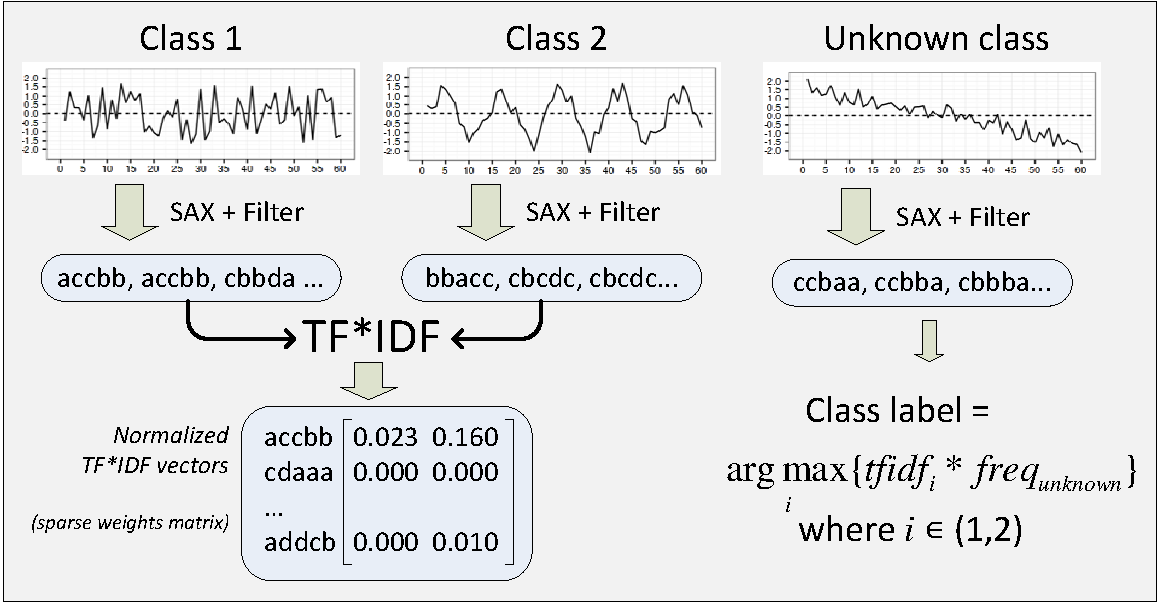
\includegraphics[width=90mm]{figures/overview.eps}
   \caption{
   An overview of SAX-VSM algorithm: 
   at first, labeled time series are converted into bags of words using SAX; 
   secondly, \textit{tf$\ast$idf} statistics is computed resulting in 
   a single weight vector per training class. For classification, an unlabeled 
   time series is converted into a term frequency vector and assigned a 
   label of a weight vector which yields a maximal cosine similarity value.
   This is \textit{ltc.nnn} weighting schema in SMART notation \cite{logtf}.}
   \label{fig:overview}
\end{figure}

\subsection{Training phase}
The training starts by transforming all of labeled time series into SAX representation
configured by three parameters: the sliding window length (\textit{W}), 
the number of PAA segments per window (\textit{P}), 
and SAX alphabet size (\textit{A}).
Each of subsequences extracted with overlapping sliding window 
is normalized (Sec. \ref{section-sax}) before being processed with PAA. 
However, if the standard deviation value falls below a fixed threshold, the 
normalization is not applied in order to avoid over-amplification 
of a background noise \cite{sax}. 

By applying this procedure to all time series from $N$ training classes, 
algorithm builds a corpus of $N$ bags, to which, in turn, 
it applies \textit{tf$\ast$idf} weighting and outputs $N$ real-valued weight 
vectors of equal length representing training classes. 

Because of the need to process the whole of the training set, 
training of SAX-VSM classifier is relatively computationally expensive ($O(nm)$). 
However, there is no need to maintain an index of training time series, 
or to keep any of them in the memory at the runtime: 
the algorithm simply iterates over all training time series incrementally building 
bags of SAX words. Once built and weighted with \textit{tf$\ast$idf}, 
the corpus is discarded - only a resulting set of $N$ real-valued weight vectors 
is retained for classification. 

\subsection{Classification}
In order to classify an unlabeled time series, SAX-VSM transforms it into a
terms frequency vector using exactly the same sliding window technique 
and SAX parameters that were used for training. 
Then, it computes cosine similarity values between this term frequency vector 
and $N$ \textit{tf$\ast$idf} weight vectors representing the training classes. 
The unlabeled time series is assigned to the class whose vector yields the
maximal cosine similarity value.

\subsection{Sliding window size and SAX parameters selection} \label{section-direct}
As shown, SAX-VSM requires three parameters to be specified upfront. 
In order to optimize their selection using only a training data set, we propose a solution based 
on a common cross-validation and DIRECT optimization scheme \cite{direct-original}.
Since DIRECT is designed to search for global minima of a real valued function 
over a bound constrained domain, we use the rounding of a reported solution values 
to the nearest integer.

DIRECT iteratively performs two procedures - partitioning the search domain and identifying 
potentially optimal hyper-rectangles.
In our case, it begins by scaling the search domain to a 3-dimensional unit hypercube 
which is considered as potentially optimal. 
The error function is then evaluated at the center of this hypercube. Next, other points are 
created at one-third of the distance from the center in all coordinate directions. 
The hypercube is then divided into smaller rectangles that are identified by their center point 
and their error function value. This procedure continues interactively until error function
converges.
For brevity, we omit the detailed explanation of the algorithm, and refer the 
interested reader to \cite{direct} for additional details. Figure \ref{fig:direct-sampling} 
illustrates the application of leave-one-out cross-validation and DIRECT to 
\textit{SyntheticControl} data set, in this case, algorithm converged after sampling 
just 130 out of 13'860 points (\textgreater100x speedup).

\begin{figure}[t]
   \centering
   \vspace{-0.2cm}
   \includegraphics[width=90mm]{figures/figure_direct.eps}
   \caption{Parameters optimization with DIRECT for \textit{SyntheticControl} data. 
   Left panel shows all points sampled by DIRECT in the space $PAA*Window*Alphabet$ where
   red points correspond to high error values in cross-validation experiments, 
   while green points indicate low error values. 
   Note the green points concentration at $W$=42. 
   Middle panel shows an error rate heat map of a hypercube slice ($W$ is fixed to 42)
   obtained by a complete scan of all 432 points. 
   Right panel shows an error rate heat map of the same slice when 
   the sampling process optimized by DIRECT, 
   the optimal solution ($P$=8,$A$=4) was found by sampling of 43 points.}
   \vspace{-0.1cm}
   \label{fig:direct-sampling}
\end{figure}

\section{Results} \label{results}
We have proposed a novel algorithm for time series classification based on SAX
approximation of time series and Vector Space Model called SAX-VSM. 
Here, we present a range of experiments assessing its performance and showing
its ability to provide an insight into classification results.

\subsection{Analysis of the classification accuracy}
We evaluated our approach on 45 datasets whose majority was taken from benchmark 
data disseminated through UCR repository \cite{ucr}. While all the detail are available at 
project's homepage \cite{jmotif}, Table \ref{perf_table} compares the classification accuracy 
of SAX-VSM with previously published performance results of four competing classifiers: 
two state-of-the-art 1NN classifiers based on Euclidean distance and DTW, 
the classifier based on recently proposed Fast-Shapelets technique \cite{fast-shapelets}, 
and the classifier based on BOP \cite{bag_patterns}.
We selected these particular techniques in order to position SAX-VSM in terms of 
classification accuracy and interpretability. 

In our evaluation, we followed a train/test data split as provided by UCR. 
Train data were used in cross-validation experiments for optimization of 
SAX parameters using \mbox{DIRECT}. 
Once selected, optimal parameters were used to assess SAX-VSM classification 
accuracy on test data which is reported in the last column of Table \ref{perf_table}.

\begin{footnotesize}
\begin{table}[t]
\vspace{-0.3cm}
\caption{\bf Classifiers error rates comparison.}
 \label{perf_table}
\centering
\begin{tabularx}{\linewidth}{@{} l *6X @{}}
\hline
Dataset & Nb. of classes & 1NN-Euclidean & 1NN-DTW & Fast Shapelets &  \mbox{Bag Of} \mbox{Patterns}
& SAX-VSM\\
\hline
Adiac        &37  & 0.389   & 0.391  & 0.514  & 0.432  & \textbf{0.381}\\
Beef         &5   & 0.467   & 0.467  & 0.447  & 0.433  & \textbf{0.033}\\
CBF         & 3  & 0.148    & 0.003  & 0.053    & 0.013 & \textbf{0.002} \\
Coffee       &2    & 0.250   & 0.180  & 0.067     & 0.036     & \textbf{0.0} \\
ECG200     &2   & \textbf{0.120}  & 0.230  & 0.227     & 0.140   & 0.140 \\
FaceAll      &14  & 0.286   & \textbf{0.192}  & 0.402     & 0.219   & 0.207\\
FaceFour    &4   & 0.216   & 0.170  & 0.089     & 0.011   & \textbf{0.0} \\
Fish         &7   & 0.217   & 0.167  & 0.197    & 0.074   & \textbf{0.017} \\
Gun-Point    &2   & 0.087   & 0.093  & 0.060     & 0.027     & \textbf{0.007} \\
Lightning2    &2   & 0.246   & \textbf{0.131}  & 0.295  & 0.164  & 0.196 \\
Lightning7    &7   & 0.425   & \textbf{0.274}  & 0.403  & 0.466  & 0.301 \\
Olive Oil     &4   & 0.133   & 0.133  & 0.213     & 0.133  & \textbf{0.100}\\
OSU Leaf    &6   & 0.483   & 0.409  & 0.359     & 0.236  & \textbf{0.107} \\
Syn.Control  &6   & 0.120   & \textbf{0.007}  & 0.081     & 0.037  & 0.010 \\
Swed.Leaf   &15  & 0.213   & 0.210 & 0.270 & \textbf{0.198} & 0.251 \\
Trace       &4   & 0.240   & \textbf{0.0}    & 0.002  & \textbf{0.0} & \textbf{0.0} \\
Two patterns &4   & 0.090   & \textbf{0.0}    & 0.113   & 0.129      & 0.004 \\
Wafer        &2    & 0.005   & 0.020     & 0.004  & 0.003 & \textbf{0.0006} \\
Yoga        &2    & 0.170   & \textbf{0.164}  & 0.249 & 0.170 & \textbf{0.164} \\
\hline
\vspace{0.1cm}
\end{tabularx}
\end{table}
\end{footnotesize}

\subsection{Scalability analysis} \label{scalability}
For synthetic datasets, it is possible to create as many time series instances as 
one needs for experimentation.
We used CBF \cite{cbf} domain in order to investigate and assess the performance 
of SAX-VSM on increasingly large datasets.

In one series of experiments, we varied a training set size from 10 to $10^{3}$, while 
the test set size remained fixed to $10^{4}$ instances. 
For small training sets, SAX-VSM was found to be significantly more accurate than 
1NN Euclidean classifier, but by the time we had more than 500 time series in a training set, 
there was no significant difference in accuracy (Fig. \ref{fig:precision-runtime}, left). 
As per the runtime cost, due to the comprehensive training, SAX-VSM was found to 
be more expensive than 1NN Euclidean classifier on small training sets, 
but outperformed 1NN on large training sets. Note that SAX-VSM allows to perform training 
offline and load weight vectors when needed - in this scenario, it performs classification 
significantly faster than 1NN Euclidean classifier (Fig. \ref{fig:precision-runtime}, right).

In another series of experiments we investigated the scalability of our algorithm with
unrealistic training set sizes - up to $\normalsize{10^{9}}$ of instances of each of CBF classes.
As expected, with the grows of a training set size, the growth curve of a total number of 
distinct SAX words for each class' dictionary showed significant saturation 
(similar to logarithmic curve) peaking at about 10\% of all possible words for selected 
PAA and alphabet sizes.
This result reflects SAX-VSM ability to learn efficiently from large datasets: 
while SAX smoothing limits the generation of new words corresponding to 
relatively similar sub-sequences, the \textbf{\textit{idf}} factor of the weighting 
schema (Eq. \ref{formula:idf}) efficiently prunes SAX words (patterns) 
that are loosing their discriminative power, i.e. those which appear in all classes.

\begin{figure}[b]
   \centering
   \vspace{0.4cm}
   \includegraphics[width=88mm]{figures/precision-runtime_new.eps}
   \caption{Comparison of classification precision and run time of SAX-VSM and 1NN 
   Euclidean classifier on CBF data. 
   Left: SAX-VSM performs significantly better with limited amount of training samples. 
   Center: while SAX-VSM is faster in time series classification, its performance 
   is comparable to 1NN Euclidean when training time is accounted for.
   Right: SAX-VSM increasingly outperforms 1NN Euclidean with noise level growth 
   (the random noise level varies up to 100\% of CBF signal value)
   }
   \label{fig:precision-runtime}
   \vspace{-0.45cm}
\end{figure}

%dictionary of the
%with While it grows rapidly at the beginning, once
%the dictionary is saturated, growth tend to slow down (left panel of Figure \ref{fig:corrupted}). 
%Nevertheless, by adjusting alphabet and PAA sizes it is possible to keep the number of terms
%significantly large. 
%\begin{figure}[t]
   %\myfigureshrinker
   %\centering
   %\includegraphics[width=84mm]{figures/Bubbles.eps}
   %\caption{Left panel: illustration of dictionaries size evolution for CBF with
   %increasingly large training set size. 
   %Right panel: distribution of SAX terms in CBF corpus for training set of 
   %one million series of each class.}
   %\label{fig:venn}
%\end{figure}

\subsection{Robustness to noise}
Since the weight of each of the overlapping SAX words is contributing only a small 
fraction to a final similarity value, we hypothesized that SAX-VSM classifier might be 
robust to the noise and to the partial loss of a signal in test time series. 
Intuitively, in this case the cosine similarity between high dimensional 
weight vectors might not degrade significantly enough to cause a misclassification.

We investigated this hypothesis using CBF data. By fixing a training set size to 250 
time series, we varied the standard deviation of Gaussian noise in CBF model.
SAX-VSM outperformed 1NN Euclidean classifier with the growth of a noise level 
confirming our hypothesis (Fig.\ref{fig:precision-runtime}). 
Further improvement of SAX-VSM performance was achieved by fine tuning of smoothing 
through a gradual increase of the SAX sliding window size proportionally to the growth of 
the noise level (\textit{SAX-VSM Opt} curve, Fig.\ref{fig:precision-runtime}). 

\begin{figure}[b]
   %\myfigureshrinker
   \centering
   \vspace{0.3cm}
   \includegraphics[width=88mm]{figures/CBF-HEAT.eps}
   \caption{An example of the heat map-like visualization of subsequence ``importance''
   to a class identification. Color value of each point was obtained by combining 
   \textit{tf$\ast$idf} weights of all patterns which cover the point.
   Highlighted by the visualization features correspond to a sudden rise, plateau, 
   and a sudden drop in Cylinder; increasing trend in Bell; and to a sudden rise 
   followed by a gradual drop in Funnel, align exactly with CBF design \cite{cbf}.}
   \label{fig:heat}
   \vspace{-0.5cm}
\end{figure}

\subsection{Interpretable classification}
While the classification performance evaluation results show that SAX-VSM classifier has 
a very good potential, its major strength is in the level of allowed interpretability of 
classification results. 

Previously it was shown that shapelet-based decision trees provide interpretable 
classification and offer an insight into underlying data features \cite{shapelet}. 
Later, it was shown that the discovery of multiple shapelets provides even 
better resolution and intuition into the interpretability of classification \cite{bagnal}. 
However, as the authors noted, the time cost of multiple shapelets discovery
in many class problems could be very significant. 
In contrast, SAX-VSM extracts and weights all patterns at once without
any added cost. Thus, it could be the only choice for interpretable classification 
in many class problems. 
Here, we show a few examples in which we exploit the subsequence weighting 
provided by our technique.

\subsubsection{Heatmap-like visualization}
Since SAX-VSM outputs tf$\ast$idf weight vectors of all subsequences extracted from a
class, it is possible to find out a weight of any arbitrary selected subsequence.
This feature enables a novel heat map-like visualization technique that provides an immediate
insight into the layout of ``important'' class-characterizing subsequences 
as shown at Figure \ref{fig:heat}.

\begin{figure}[]
   %\myfigureshrinker
   \centering
   \includegraphics[width=87mm]{figures/gun-point.eps}
   \caption{Best characteristic subsequences (right panels, bold lines) discovered by 
   SAX-VSM in \textit{Gun/Point} dataset. 
   Left panels show actor's stills and time series annotations made by an expert, 
   right panels show locations of characteristic subsequences.
   Note, that while the upward arm motion is found to be more ``important'' in \textit{Gun} 
   class (gun retrieval and aiming), the downward arm motion better characterizes 
   \textit{Point} class (an ``overshoot'' phenomena in propless arm return). 
   This result aligns with previous work \cite{shapelet} and \cite{bagnal}.
   (Stills and annotation used with a permission from E. Keogh) }
   \label{fig:shapelet-like-patterns}
   \vspace{-0.2cm}
\end{figure}

\subsubsection{Gun Point dataset}
Following previous shapelet-based work \cite{shapelet} \cite{bagnal}, 
we used a well-studied \textit{GunPoint} dataset \cite{gun} to explore the 
interpretability of classification results. The class \textit{Gun} of this dataset 
corresponds to the actors' hands motion when drawing a replicate gun from 
a hip-mounted holster, pointing it at a target for a second, and returning the 
gun to the holster; class \textit{Point} correspond to the actors hands motion 
when pretending of drawing a gun - the actors point their index fingers to 
a target for about a second, and then return their hands to their sides. 

Similarly to previously reported results, SAX-VSM was able to capture all 
distinguishing features as shown at the Figure \ref{fig:shapelet-like-patterns}. 
The top weighted by SAX-VSM patterns in \textit{Gun} class corresponds 
to fine movements required to lift and aim the prop. 
The top weighted SAX pattern in \textit{Point} class corresponds to the 
``overshoot'' phenomena causing the dip in the time series \cite{gun}, 
while the second to best pattern captures the lack of movements
required for lifting a hand above a holster and reaching down for the prop. 

\subsubsection{OSU Leaf dataset}
The \textit{OSULeaf} dataset consist of curves obtained by color image segmentation 
and boundary extraction from digitized leaf images of six classes \cite{osuleaf}.
The author was able to solve the problem of leaf boundary curves classification 
with DTW, achieving 61\% of classification accuracy. 
However, DTW provided a very little information about why it succeeded of failed,
whereas SAX-VSM application yielded a set of class-specific characteristic 
patterns for each of six classes which match closely known techniques 
for leaves classification based on a leaf shape\cite{dirr}. 
Highlighted by SAX-VSM features include the slightly lobed shape and acute tips of
Acer Circinatum, serrated blade of Acer Glabrum, and the acuminate tip and characteristic
serration of in Acer Macrophyllum leaves, pinnately compound leaves arrangement of Acer Negundo, the
incised leaf margin of Quercus Kelloggii, and a lobed leaf structure of Quercus Garryana 
(Figure \ref{fig:shapelet-acer-patterns}).

\begin{figure}[t]
   %\myfigureshrinker
   \centering
   \vspace{-0.2cm}
   \includegraphics[width=87mm]{figures/AcerCircunatum-short.eps}
   \caption{Example of best characteristic subsequences (top panels, bold lines) discovered 
   by SAX-VSM in \textit{OSULeaf dataset}.
    These patterns align exactly with known in botany discrimination techniques based on lobe shapes, 
    serrations, and leaf tip types \cite{dirr}.}
   \label{fig:shapelet-acer-patterns}
   \vspace{-0.2cm}
\end{figure}

\subsubsection{Coffee dataset}
Similarly to the original work based on PCA \cite{coffee}, SAX-VSM highlighted intervals 
corresponding to Chlorogenic acid (best) and Caffeine (second to best) 
in both classes of Coffee spectrograms. These two chemical compounds that are 
known to be responsible for the flavor differences in Arabica and Robusta coffees.

\section{Conclusion and Future Work} \label{conclusion}
In this paper, we have proposed a novel interpretable technique for time series classification
based on characteristic patterns discovery. We have shown, that our approach is competitive with, 
or superior to, other techniques on a set of classic data mining problems. In addition, 
we described several advantages of SAX-VSM over existing structure-based similarity measures,
emphasizing its capacity to discover and rank short subsequences by their class characterization
power. Finally, we outlined an efficient solution for SAX parameters selection.

For our future work, inspired by recently reported superior performance of multi-shapelet based 
classifiers \cite{bagnal}, we prioritize modification of our algorithm for words of variable length.
In addition, we explore SAX-VSM applicability for multidimensional time series. 

\bibliographystyle{IEEEtran}

\begin{thebibliography}{5}

%1
\bibitem {review}
Wang, X., Mueen, A., Ding, H., Trajcevski, G., Scheuermann, P., Keogh, E.:
Experimental comparison of representation methods and distance measures for time series data.
DMKD, 26, 2, 275--309 (2013)

%2
\bibitem {benchmark}
Keogh, E., Kasetty, S.:
On the need for time series data mining benchmarks: a survey and empirical demonstration.
DMKD, 7, 4, 349--371 (2003)

%3
\bibitem {classifiers}
Salzberg, S.:
On comparing classifiers: Pitfalls to avoid and a recommended approach. 
DMKD, 1, 317--328 (1997)

%4
\bibitem {comparison}
Ding, H., Trajcevski, G., Scheuermann, P., Wang, X., Keogh, E.:
Querying and mining of time series data: experimental comparison of representations and distance
measures. 
In Proc. VLDB, 1542--1552 (2008)

%5
\bibitem {1NN}
Xi, X., Keogh, E., Shelton, C., Wei, L., Ratanamahatana, C.:
Fast time series classification using numerosity reduction. 
In Proc. ICML, 1033--1040 (2006)

%6
\bibitem {DTW}
Sakoe, H. Chiba, S.:
Dynamic programming algorithm optimization for spoken word recognition.
IEEE Trans. on Acoustics, Speech and Signal Processing, 1, 43--49 (1978)

%7
\bibitem {DFT}
Agrawal, R., Faloutsos, C., Swami, A.:
Efficient Similarity Search In Sequence Databases.
In Proc. FODO, 69--84 (1993)

%8
\bibitem {bag_patterns}
Lin, J., Khade, R., Li, Y.:
Rotation-invariant similarity in time series using bag-of-patterns representation. 
J. Intell. Inf. Syst. 39, 2, 287--315 (2012)

%9
\bibitem {shapelet}
Ye, L., Keogh, E.:
Time series shapelets: a novel technique that allows accurate, interpretable and fast
classification. 
DMKD, 22, 149--182 (2011)

%10
\bibitem {bagnal}
Lines, J., Davis, L., Hills, J., Bagnall, A.:
A shapelet transform for time series classification. 
In Proc. 18th ACM SIGKDD, 289--297 (2012)

%11
\bibitem {fast-shapelets}
Rakthanamanon, T., Keogh, E.:
Fast-Shapelets: A Scalable Algorithm for Discovering Time Series Shapelets.
In Proc. SDM (2013)

%12
\bibitem {sax}
Lin, J., Keogh, E., Wei, L., Lonardi, S.:
Experiencing SAX: a novel symbolic representation of time series.
DMKD, 107--144 (2007)

%13
\bibitem {salton}
Salton, G., Wong, A., Yang., C.:
A vector space model for automatic indexing. 
Commun. ACM 18, 11, 613--620 (1975)

%14
\bibitem {direct}
Bj\"{o}rkman, M., Holmstr\"{o}m, K.:
Global Optimization Using the DIRECT Algorithm in Matlab.
Adv. Modeling and Optimization, 1, 17-37 (1999)

%15
\bibitem {hot_sax}
Keogh, E., Lin, J., Fu, A.:
HOT SAX: Efficiently Finding the Most Unusual Time Series Subsequence. 
In Proc. ICDM. 226--233 (2005)

%16
\bibitem {goldin_kanellakis}
Goldin D., Kanellakis, P.:
On Similarity Queries for Time-Series Data: Constraint Specification and Implementation. 
In Proc CP. 137--153 (1995)

%17
\bibitem {paa}
Keogh, E., Pazzani, M.:
A Simple Dimensionality Reduction Technique for Fast Similarity Search in Large Time Series
Databases. In Proc. PADKK, 122--133 (2000)

%18
\bibitem {logtf}
Manning, C., Raghavan, P., Sch\"utze, H.: 
Introduction to Information Retrieval, Cambridge University Press (2008)

%19
\bibitem {direct-original}
Jones, D., Perttunen, C., Stuckman, B.:
Lipschitzian Optimization without Lipschitz Constant.
J. Optim. Theory Appl. 79, 1 (1993)

%20
\bibitem {ucr}
Keogh, E., Zhu, Q., Hu, B., Hao, Y.,  Xi, X., Wei, L., Ratanamahatana, C.:
The UCR Time Series Classification/Clustering Homepage:
\url{http://www.cs.ucr.edu/~eamonn/time_series_data/}

%21
\bibitem {jmotif}
Paper authors. Supporting webpage:
\url{https://code.google.com/p/jmotif/}

%22
\bibitem {cbf}
Saito, N:
Local feature extraction and its application using a library of bases. 
PhD thesis, Yale University (1994)

%23
\bibitem {gun}
Ratanamahatana, C., Keogh, E.:
Making time-series classification more accurate using learned constraints. 
In SDM '04 (2004)

%24
\bibitem {osuleaf}
Gandhi, A.:
Content-Based Image Retrieval: Plant Species Identification. 
MS thesis, Oregon State University (2002)

%25
\bibitem {dirr}
Dirr, M.:
Manual of Woody Landscape Plants: Their Identification, Ornamental Characteristics,
Culture, Propogation and Uses.
Stipes Pub Llc, ed. 6 Revised (2009)

%26
\bibitem {coffee}
Briandet, R., Kemsley, E., Wilson, R.:
Discrimination of Arabica and Robusta in Instant Coffee by Fourier Transform Infrared Spectroscopy
and Chemometrics.
J. Agric. Food Chem, 44, 170--174 (1996)

\end{thebibliography}

\begin{figure}[t]
   %\myfigureshrinker
   \centering
   \vspace{-0.2cm}
   \includegraphics[width=84mm]{figures/coffee_patterns.ps}
   \caption{
   Best characteristic subsequences (left panels, bold lines) discovered by SAX-VSM in
   {Coffee dataset}. Right panels show zoom-in view on these subsequences in Arabica
   and Robusta spectrograms.
   These discriminative subsequences correspond to chlorogenic acid (best subsequence) 
   and to caffeine (second to best) regions of spectra. This result aligns with
   the original work based on PCA \cite{coffee} exactly.
   %Best characteristic subsequences discovered by SAX-VSM in \textit{Coffee data set}.
   %The best subsequences in both classes correspond to chlorogenic acid, while
   %second to best subsequences - to caffeine. This result aligns with previous 
   %exploratory research based on PCA \cite{coffee}.
   }
   \label{fig:coffee}
   \vspace{-0.2cm}
\end{figure}

% that's all folks
\end{document}
